\documentclass[journal,compsoc, 10pt, draftclsnofoot, onecolumn]{IEEEtran}

\usepackage{graphicx}
\usepackage{amssymb}
\usepackage{amsmath}
\usepackage{amsthm}
\usepackage{tabularx}
\usepackage{graphicx}

\newcommand{\subparagraph}{}
\usepackage{titlesec}

\usepackage{alltt}
\usepackage{float}
\usepackage{color}
\usepackage{url}

\usepackage{balance}
\usepackage[TABBOTCAP, tight]{subfigure}
\usepackage{enumitem}
\usepackage{pstricks, pst-node}

\usepackage{cite}
\usepackage{listings}
\usepackage{placeins}

\usepackage[margin=0.75in]{geometry}
\geometry{textheight=8.5in, textwidth=6in}

\renewcommand{\familydefault}{\sfdefault}

\newlength\tindent
\setlength{\tindent}{\parindent}
\setlength{\parindent}{0pt}
\renewcommand{\indent}{\hspace*{\tindent}}

\newcommand{\cred}[1]{{\color{red}#1}}
\newcommand{\cblue}[1]{{\color{blue}#1}}

\newcommand{\namesigdate}[2][6cm]{%
  \begin{tabular}{@{}p{#1}@{}}
    #2 \\[0.5\normalbaselineskip] \hrule \\[0.pt]
    {\small \vspace{-3em} \textit{Signature}} \\[0.5\normalbaselineskip] \hrule \\[0pt]
    {\small \vspace{-3em}\textit{Date}}
  \end{tabular}
}


\usepackage{hyperref}
\usepackage{geometry}

\lstset{
language=C,
basicstyle=\ttfamily,
commentstyle=\color{blue},
numberstyle=\color{red},
stringstyle=\color{orange}
}

\def\nameD{Devin Foulger}

\usepackage{fancyvrb}
\usepackage{color}
\usepackage[latin1]{inputenc}


\makeatletter
\def\PY@reset{\let\PY@it=\relax \let\PY@bf=\relax%
    \let\PY@ul=\relax \let\PY@tc=\relax%
    \let\PY@bc=\relax \let\PY@ff=\relax}
\def\PY@tok#1{\csname PY@tok@#1\endcsname}
\def\PY@toks#1+{\ifx\relax#1\empty\else%
    \PY@tok{#1}\expandafter\PY@toks\fi}
\def\PY@do#1{\PY@bc{\PY@tc{\PY@ul{%
    \PY@it{\PY@bf{\PY@ff{#1}}}}}}}
\def\PY#1#2{\PY@reset\PY@toks#1+\relax+\PY@do{#2}}

\expandafter\def\csname PY@tok@gd\endcsname{\def\PY@tc##1{\textcolor[rgb]{0.63,0.00,0.00}{##1}}}
\expandafter\def\csname PY@tok@gu\endcsname{\let\PY@bf=\textbf\def\PY@tc##1{\textcolor[rgb]{0.50,0.00,0.50}{##1}}}
\expandafter\def\csname PY@tok@gt\endcsname{\def\PY@tc##1{\textcolor[rgb]{0.00,0.25,0.82}{##1}}}
\expandafter\def\csname PY@tok@gs\endcsname{\let\PY@bf=\textbf}
\expandafter\def\csname PY@tok@gr\endcsname{\def\PY@tc##1{\textcolor[rgb]{1.00,0.00,0.00}{##1}}}
\expandafter\def\csname PY@tok@cm\endcsname{\let\PY@it=\textit\def\PY@tc##1{\textcolor[rgb]{0.25,0.50,0.50}{##1}}}
\expandafter\def\csname PY@tok@vg\endcsname{\def\PY@tc##1{\textcolor[rgb]{0.10,0.09,0.49}{##1}}}
\expandafter\def\csname PY@tok@m\endcsname{\def\PY@tc##1{\textcolor[rgb]{0.40,0.40,0.40}{##1}}}
\expandafter\def\csname PY@tok@mh\endcsname{\def\PY@tc##1{\textcolor[rgb]{0.40,0.40,0.40}{##1}}}
\expandafter\def\csname PY@tok@go\endcsname{\def\PY@tc##1{\textcolor[rgb]{0.50,0.50,0.50}{##1}}}
\expandafter\def\csname PY@tok@ge\endcsname{\let\PY@it=\textit}
\expandafter\def\csname PY@tok@vc\endcsname{\def\PY@tc##1{\textcolor[rgb]{0.10,0.09,0.49}{##1}}}
\expandafter\def\csname PY@tok@il\endcsname{\def\PY@tc##1{\textcolor[rgb]{0.40,0.40,0.40}{##1}}}
\expandafter\def\csname PY@tok@cs\endcsname{\let\PY@it=\textit\def\PY@tc##1{\textcolor[rgb]{0.25,0.50,0.50}{##1}}}
\expandafter\def\csname PY@tok@cp\endcsname{\def\PY@tc##1{\textcolor[rgb]{0.74,0.48,0.00}{##1}}}
\expandafter\def\csname PY@tok@gi\endcsname{\def\PY@tc##1{\textcolor[rgb]{0.00,0.63,0.00}{##1}}}
\expandafter\def\csname PY@tok@gh\endcsname{\let\PY@bf=\textbf\def\PY@tc##1{\textcolor[rgb]{0.00,0.00,0.50}{##1}}}
\expandafter\def\csname PY@tok@ni\endcsname{\let\PY@bf=\textbf\def\PY@tc##1{\textcolor[rgb]{0.60,0.60,0.60}{##1}}}
\expandafter\def\csname PY@tok@nl\endcsname{\def\PY@tc##1{\textcolor[rgb]{0.63,0.63,0.00}{##1}}}
\expandafter\def\csname PY@tok@nn\endcsname{\let\PY@bf=\textbf\def\PY@tc##1{\textcolor[rgb]{0.00,0.00,1.00}{##1}}}
\expandafter\def\csname PY@tok@no\endcsname{\def\PY@tc##1{\textcolor[rgb]{0.53,0.00,0.00}{##1}}}
\expandafter\def\csname PY@tok@na\endcsname{\def\PY@tc##1{\textcolor[rgb]{0.49,0.56,0.16}{##1}}}
\expandafter\def\csname PY@tok@nb\endcsname{\def\PY@tc##1{\textcolor[rgb]{0.00,0.50,0.00}{##1}}}
\expandafter\def\csname PY@tok@nc\endcsname{\let\PY@bf=\textbf\def\PY@tc##1{\textcolor[rgb]{0.00,0.00,1.00}{##1}}}
\expandafter\def\csname PY@tok@nd\endcsname{\def\PY@tc##1{\textcolor[rgb]{0.67,0.13,1.00}{##1}}}
\expandafter\def\csname PY@tok@ne\endcsname{\let\PY@bf=\textbf\def\PY@tc##1{\textcolor[rgb]{0.82,0.25,0.23}{##1}}}
\expandafter\def\csname PY@tok@nf\endcsname{\def\PY@tc##1{\textcolor[rgb]{0.00,0.00,1.00}{##1}}}
\expandafter\def\csname PY@tok@si\endcsname{\let\PY@bf=\textbf\def\PY@tc##1{\textcolor[rgb]{0.73,0.40,0.53}{##1}}}
\expandafter\def\csname PY@tok@s2\endcsname{\def\PY@tc##1{\textcolor[rgb]{0.73,0.13,0.13}{##1}}}
\expandafter\def\csname PY@tok@vi\endcsname{\def\PY@tc##1{\textcolor[rgb]{0.10,0.09,0.49}{##1}}}
\expandafter\def\csname PY@tok@nt\endcsname{\let\PY@bf=\textbf\def\PY@tc##1{\textcolor[rgb]{0.00,0.50,0.00}{##1}}}
\expandafter\def\csname PY@tok@nv\endcsname{\def\PY@tc##1{\textcolor[rgb]{0.10,0.09,0.49}{##1}}}
\expandafter\def\csname PY@tok@s1\endcsname{\def\PY@tc##1{\textcolor[rgb]{0.73,0.13,0.13}{##1}}}
\expandafter\def\csname PY@tok@sh\endcsname{\def\PY@tc##1{\textcolor[rgb]{0.73,0.13,0.13}{##1}}}
\expandafter\def\csname PY@tok@sc\endcsname{\def\PY@tc##1{\textcolor[rgb]{0.73,0.13,0.13}{##1}}}
\expandafter\def\csname PY@tok@sx\endcsname{\def\PY@tc##1{\textcolor[rgb]{0.00,0.50,0.00}{##1}}}
\expandafter\def\csname PY@tok@bp\endcsname{\def\PY@tc##1{\textcolor[rgb]{0.00,0.50,0.00}{##1}}}
\expandafter\def\csname PY@tok@c1\endcsname{\let\PY@it=\textit\def\PY@tc##1{\textcolor[rgb]{0.25,0.50,0.50}{##1}}}
\expandafter\def\csname PY@tok@kc\endcsname{\let\PY@bf=\textbf\def\PY@tc##1{\textcolor[rgb]{0.00,0.50,0.00}{##1}}}
\expandafter\def\csname PY@tok@c\endcsname{\let\PY@it=\textit\def\PY@tc##1{\textcolor[rgb]{0.25,0.50,0.50}{##1}}}
\expandafter\def\csname PY@tok@mf\endcsname{\def\PY@tc##1{\textcolor[rgb]{0.40,0.40,0.40}{##1}}}
\expandafter\def\csname PY@tok@err\endcsname{\def\PY@bc##1{\setlength{\fboxsep}{0pt}\fcolorbox[rgb]{1.00,0.00,0.00}{1,1,1}{\strut ##1}}}
\expandafter\def\csname PY@tok@kd\endcsname{\let\PY@bf=\textbf\def\PY@tc##1{\textcolor[rgb]{0.00,0.50,0.00}{##1}}}
\expandafter\def\csname PY@tok@ss\endcsname{\def\PY@tc##1{\textcolor[rgb]{0.10,0.09,0.49}{##1}}}
\expandafter\def\csname PY@tok@sr\endcsname{\def\PY@tc##1{\textcolor[rgb]{0.73,0.40,0.53}{##1}}}
\expandafter\def\csname PY@tok@mo\endcsname{\def\PY@tc##1{\textcolor[rgb]{0.40,0.40,0.40}{##1}}}
\expandafter\def\csname PY@tok@kn\endcsname{\let\PY@bf=\textbf\def\PY@tc##1{\textcolor[rgb]{0.00,0.50,0.00}{##1}}}
\expandafter\def\csname PY@tok@mi\endcsname{\def\PY@tc##1{\textcolor[rgb]{0.40,0.40,0.40}{##1}}}
\expandafter\def\csname PY@tok@gp\endcsname{\let\PY@bf=\textbf\def\PY@tc##1{\textcolor[rgb]{0.00,0.00,0.50}{##1}}}
\expandafter\def\csname PY@tok@o\endcsname{\def\PY@tc##1{\textcolor[rgb]{0.40,0.40,0.40}{##1}}}
\expandafter\def\csname PY@tok@kr\endcsname{\let\PY@bf=\textbf\def\PY@tc##1{\textcolor[rgb]{0.00,0.50,0.00}{##1}}}
\expandafter\def\csname PY@tok@s\endcsname{\def\PY@tc##1{\textcolor[rgb]{0.73,0.13,0.13}{##1}}}
\expandafter\def\csname PY@tok@kp\endcsname{\def\PY@tc##1{\textcolor[rgb]{0.00,0.50,0.00}{##1}}}
\expandafter\def\csname PY@tok@w\endcsname{\def\PY@tc##1{\textcolor[rgb]{0.73,0.73,0.73}{##1}}}
\expandafter\def\csname PY@tok@kt\endcsname{\def\PY@tc##1{\textcolor[rgb]{0.69,0.00,0.25}{##1}}}
\expandafter\def\csname PY@tok@ow\endcsname{\let\PY@bf=\textbf\def\PY@tc##1{\textcolor[rgb]{0.67,0.13,1.00}{##1}}}
\expandafter\def\csname PY@tok@sb\endcsname{\def\PY@tc##1{\textcolor[rgb]{0.73,0.13,0.13}{##1}}}
\expandafter\def\csname PY@tok@k\endcsname{\let\PY@bf=\textbf\def\PY@tc##1{\textcolor[rgb]{0.00,0.50,0.00}{##1}}}
\expandafter\def\csname PY@tok@se\endcsname{\let\PY@bf=\textbf\def\PY@tc##1{\textcolor[rgb]{0.73,0.40,0.13}{##1}}}
\expandafter\def\csname PY@tok@sd\endcsname{\let\PY@it=\textit\def\PY@tc##1{\textcolor[rgb]{0.73,0.13,0.13}{##1}}}

\def\PYZbs{\char`\\}
\def\PYZus{\char`\_}
\def\PYZob{\char`\{}
\def\PYZcb{\char`\}}
\def\PYZca{\char`\^}
\def\PYZam{\char`\&}
\def\PYZlt{\char`\<}
\def\PYZgt{\char`\>}
\def\PYZsh{\char`\#}
\def\PYZpc{\char`\%}
\def\PYZdl{\char`\$}
\def\PYZti{\char`\~}
% for compatibility with earlier versions
\def\PYZat{@}
\def\PYZlb{[}
\def\PYZrb{]}
\makeatother


\hypersetup {
        colorlinks = true,
        urlcolor = black,
        linkcolor = black,
        pdfauthor = {\nameD},
        pdfkeywords = {},
        pdfsubject = {},
        pdfpagemode = UseNone
}

\titleformat{\section}
	{\normalfont\fontsize{15}{10}\bfseries}{\thesection}{1em}{}
\titleformat{\subsection}
	{\normalfont\fontsize{12}{15}\bfseries}{\thesubsection}{1em}{}
\titleformat{\subsubsection}
	{\normalfont\fontsize{12}{15}\bfseries}{\thesubsubsection}{1em}{}

\begin{document}

\title{\vspace{20em}Spring Midterm Report \\{\vspace{-1ex}\huge UniversityGear} \\
{\large \today}}
\author{\vspace{10ex}Devin Foulger \\{\vspace{-1ex}Hector Trujillo}
\\{\vspace{-1ex}Bryan Liauw}}

\begin{titlepage}

\maketitle
\thispagestyle{empty}

\begin{abstract}
This document will recap what we have done over the term and will describe 
what we plan to do in the following year. It will go into detail about the goals 
we have set and how we plan to accomplish them. It will also include a summary 
of the project status as it is now. It will also include a retrospective of what 
has happened throughout the term.
\end{abstract}

\end{titlepage}

\tableofcontents

\section{Introduction}
This term hasn't been about development. Most of our development was 
completed last term. Instead the team has been looking for bugs in the application. 
The group has also been preparing for Expo by completing the poster and prepping 
for talking points about the project.

\section{Project goals and recap}
The goal of the project is to build an Android application that will allow users 
to purchase college related merchandise. This means that users will be able to 
search for many items depending on user provided information. They can 
search for specific schools and their colors as well as condition of item, or 
the price. We also set out to accomplish how to create documents in which we 
could effectively describe our project. \newline

Here are the recaps for each week of spring term so far.

\subsection{Spring Term}
\textbf{Week 1}\newline
During the course of week 1, the purchase class was officially completed. The team 
was also able to implement a method that allows for new items to be gathered once 
the item list reached the end of the bottom. Testing has also been started.

\textbf{Week 2}\newline
During week 2, minor UI improvements had been made and bugs have been found. 
Overall, minor changes were made.

\textbf{Week 3}\newline
Testing and bug fixing was completed over week 3.

\textbf{Week 4}\newline
Over week 4, a couple of bigger bugs were fixed. The custom CSS that was being 
displayed in the description of certain items significantly increased the size of descriptions. 
This made it incredibly hard to read and it looked like something was broken. In order to 
fix this, a webview was created to render the CSS properly on another page. The 
image in the single item view was also updated so it wasn't completely stretched out.

\textbf{Week 5}\newline
Week 5 was a stressful week. This was because the completion date for our 
application had come. In order to prepare for launch, we did extensive testing to 
find any remaining bugs. 

\section{Project status}
Over the course of the term, the group has done relatively development work as 
most of that has been completed in the previous term. Minor work with the purchase 
class was finished during week 2. The group has been focusing on finding and fixing 
bugs that are remaining in the application. This means that it is now completely 
possible for the user to search for items that they want, view them, and then 
purchase them. Currently, there are two versions of the application: production 
and sandbox. The production version is using the production APIs, meaning that 
it will get live data. The sandbox version is used specifically for testing purposes. 
This version will allow someone to test every functionality of the app without 
actually having to purchase an item. 

\subsection{Purchase Class Development}
The purchase class is what will allow the user to buy an item that they have selected. 
The user needs to provide several key pieces of information, such as the credit card 
info and shipping address. The class will make use of eBay's Order API. First, the 
user must enter in all relevant information. When they click the purchase 
button, the checkout session is initiated. This is done by using the initiate 
guest checkout API call. This call needs to have the shipping address as well as 
the ID of the selected item. From there, it will then call the purchase API call, 
which will use the users credit card information to complete the purchase. \newline

In order to complete this class, three separate Http calls had to be made. One for 
initiating the purchase session, the second for adding credit card information, and 
the last for making the purchase. The purchase initiate call returned a session id that 
needed to be used in the other requests. Any data that was sent in the body of the 
http request was built in JSON format. 

\section{Impediments and solutions}
Over the course of the term so far, there was one large clocked that we 
had encountered. It was during the purchase class development that we found 
this problem. The OAuth key that we were using to try and complete the purchase 
did not correctly work. The solution was that we needed to create a separate OAuth 
token for the purchase class. In order to do this, we had to generate a new OAuth 
token with a narrower scope, meaning that the token generated could only be used 
with the purchasing class.

\section{Remaining Items}
The only remaining items are bugs that we have found.

\subsection{Known Bugs}
There are a total of four bugs remaining in our application. The first being a simple 
bug in which the categories aren't cleared from the API call after they have been 
unselected. The next bug has to do with the item class finding three items when 
only two items are actually returned. The third bug happens when multiple schools 
are selected to search for. This is because the school names are merged together 
as one string. The  last bug happens when specific return information is given. It 
displays incorrectly to the user.\newpage

\section{Project Images}
\begin{figure}[h]
This image demonstrates what is displayed to the user after they successfully 
complete a search. This will list all possible searches. Each item card will display 
the title, image and price. 
\centering
\caption{List view of items}
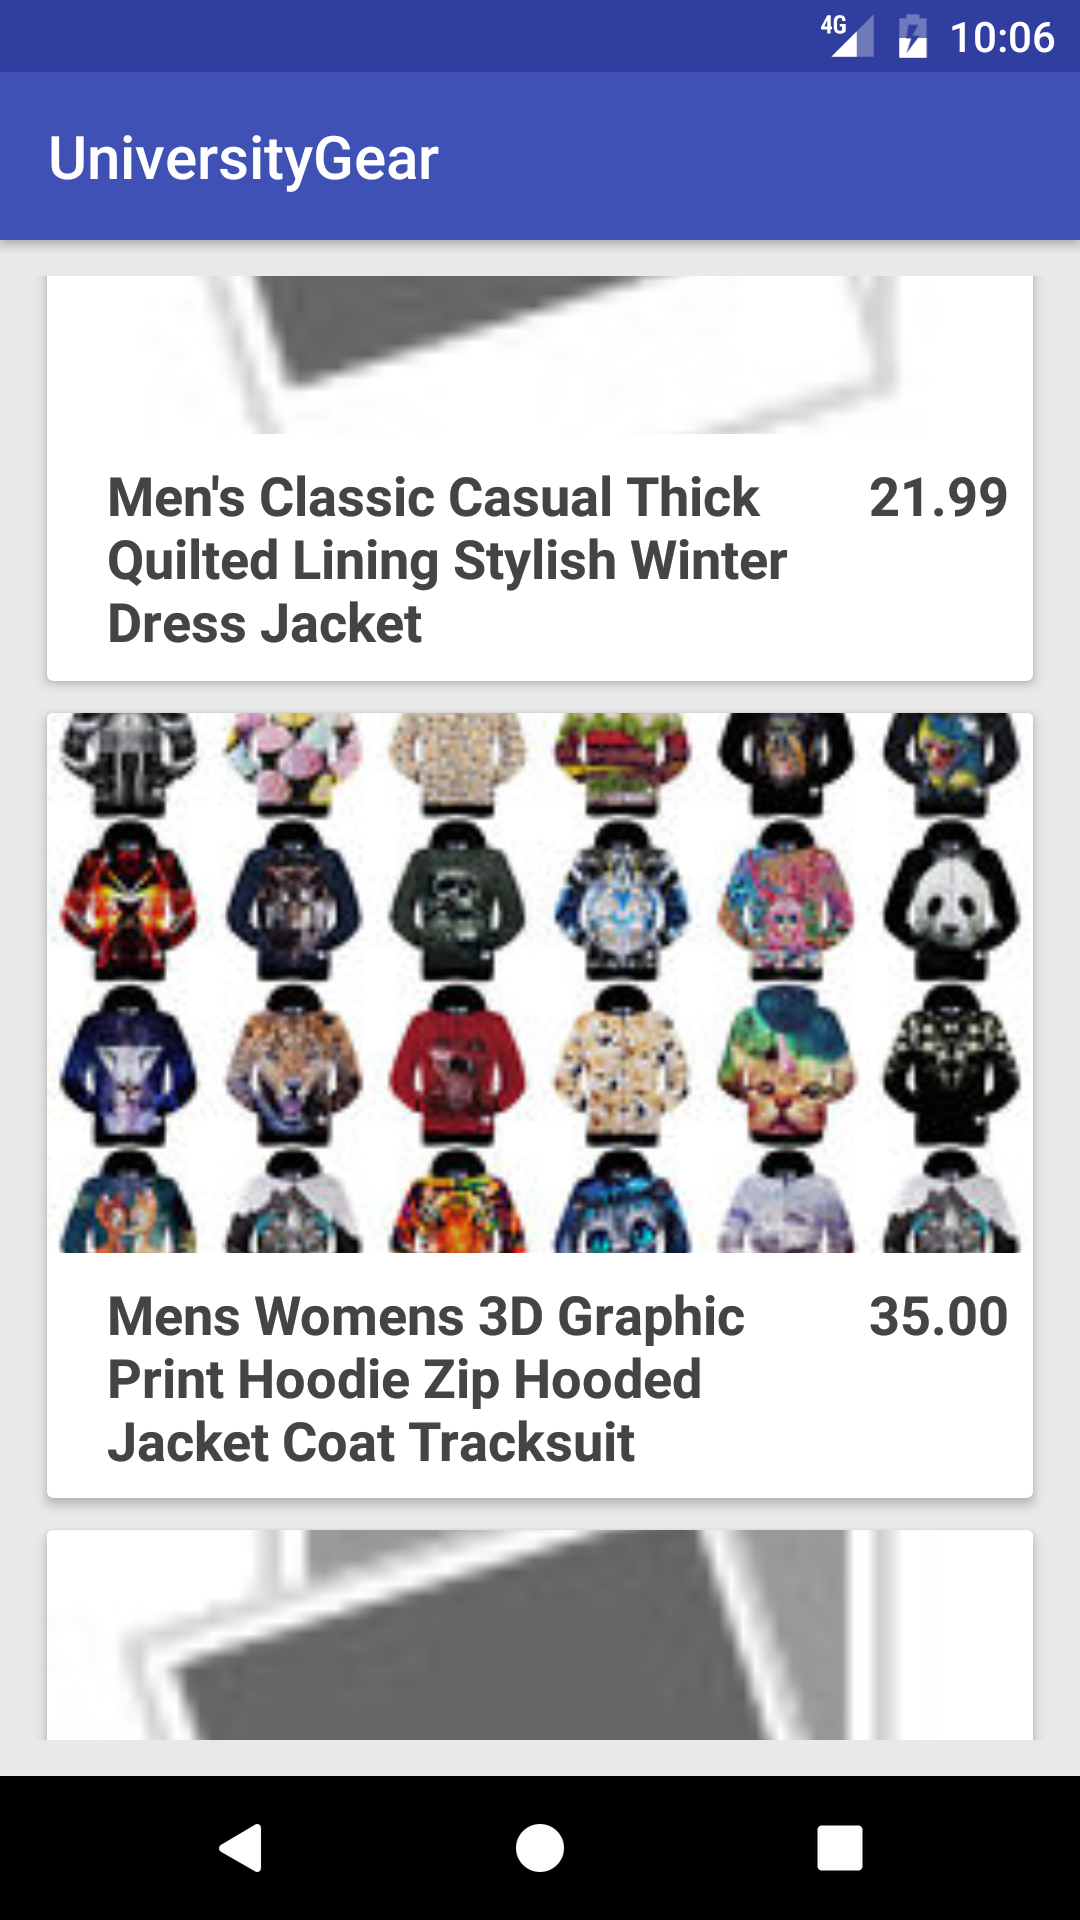
\includegraphics[scale=.2]{listview}
\end{figure}

\begin{figure}[t]
This is an image of what a single item would look like when being viewed. 
It contains the title, price, and other important information that pertains to 
the item.
\centering
\caption{Image of single item}

\includegraphics[scale=.2]{singleview1}
\end{figure}

\begin{figure}[t]
This is what the rest of the single item view would display to the user. It 
shows more details about the item as well as shipping and return info.
\centering
\caption{Item details of a single item}
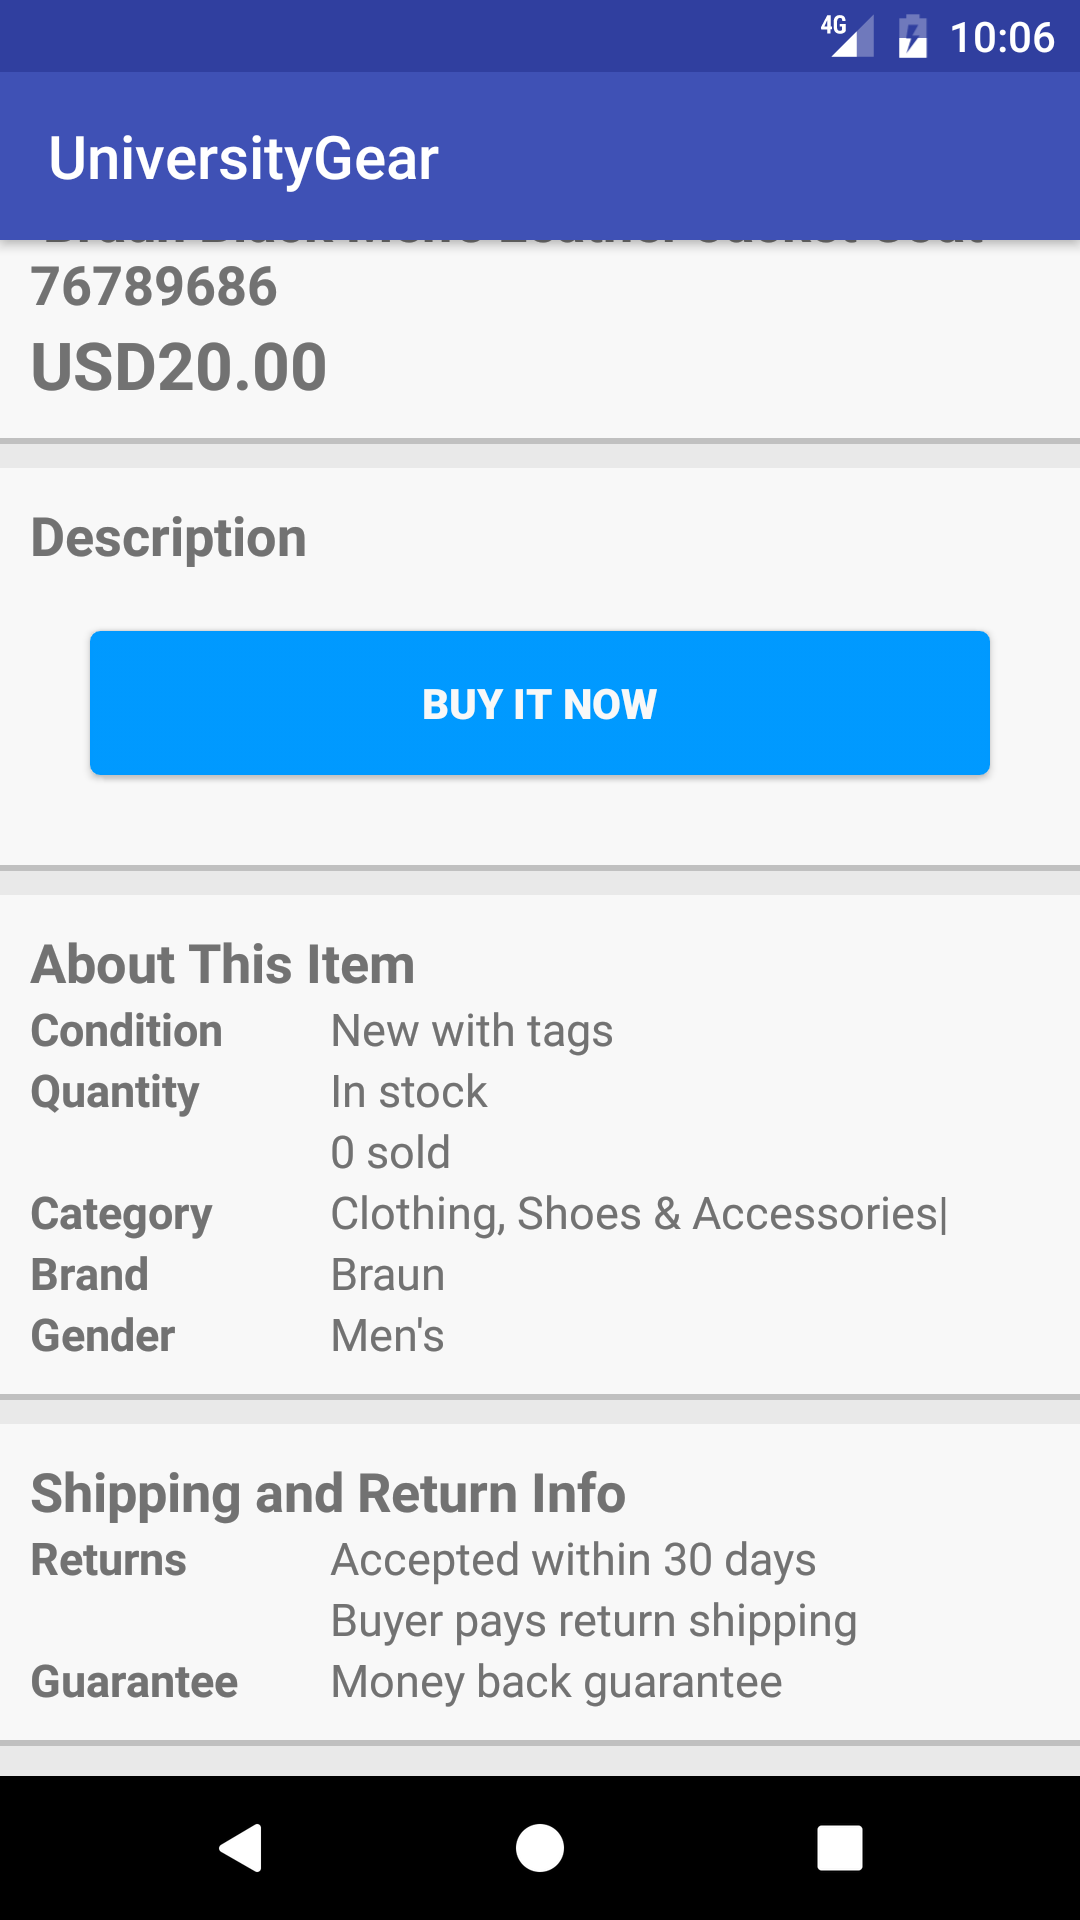
\includegraphics[scale=.2]{singleview2}
\end{figure}
\FloatBarrier

\begin{figure}[t]
This is what it looks like when the user is filling out the form to purchase the 
item they have selected.
\centering
\caption{Form for completing a purchase}
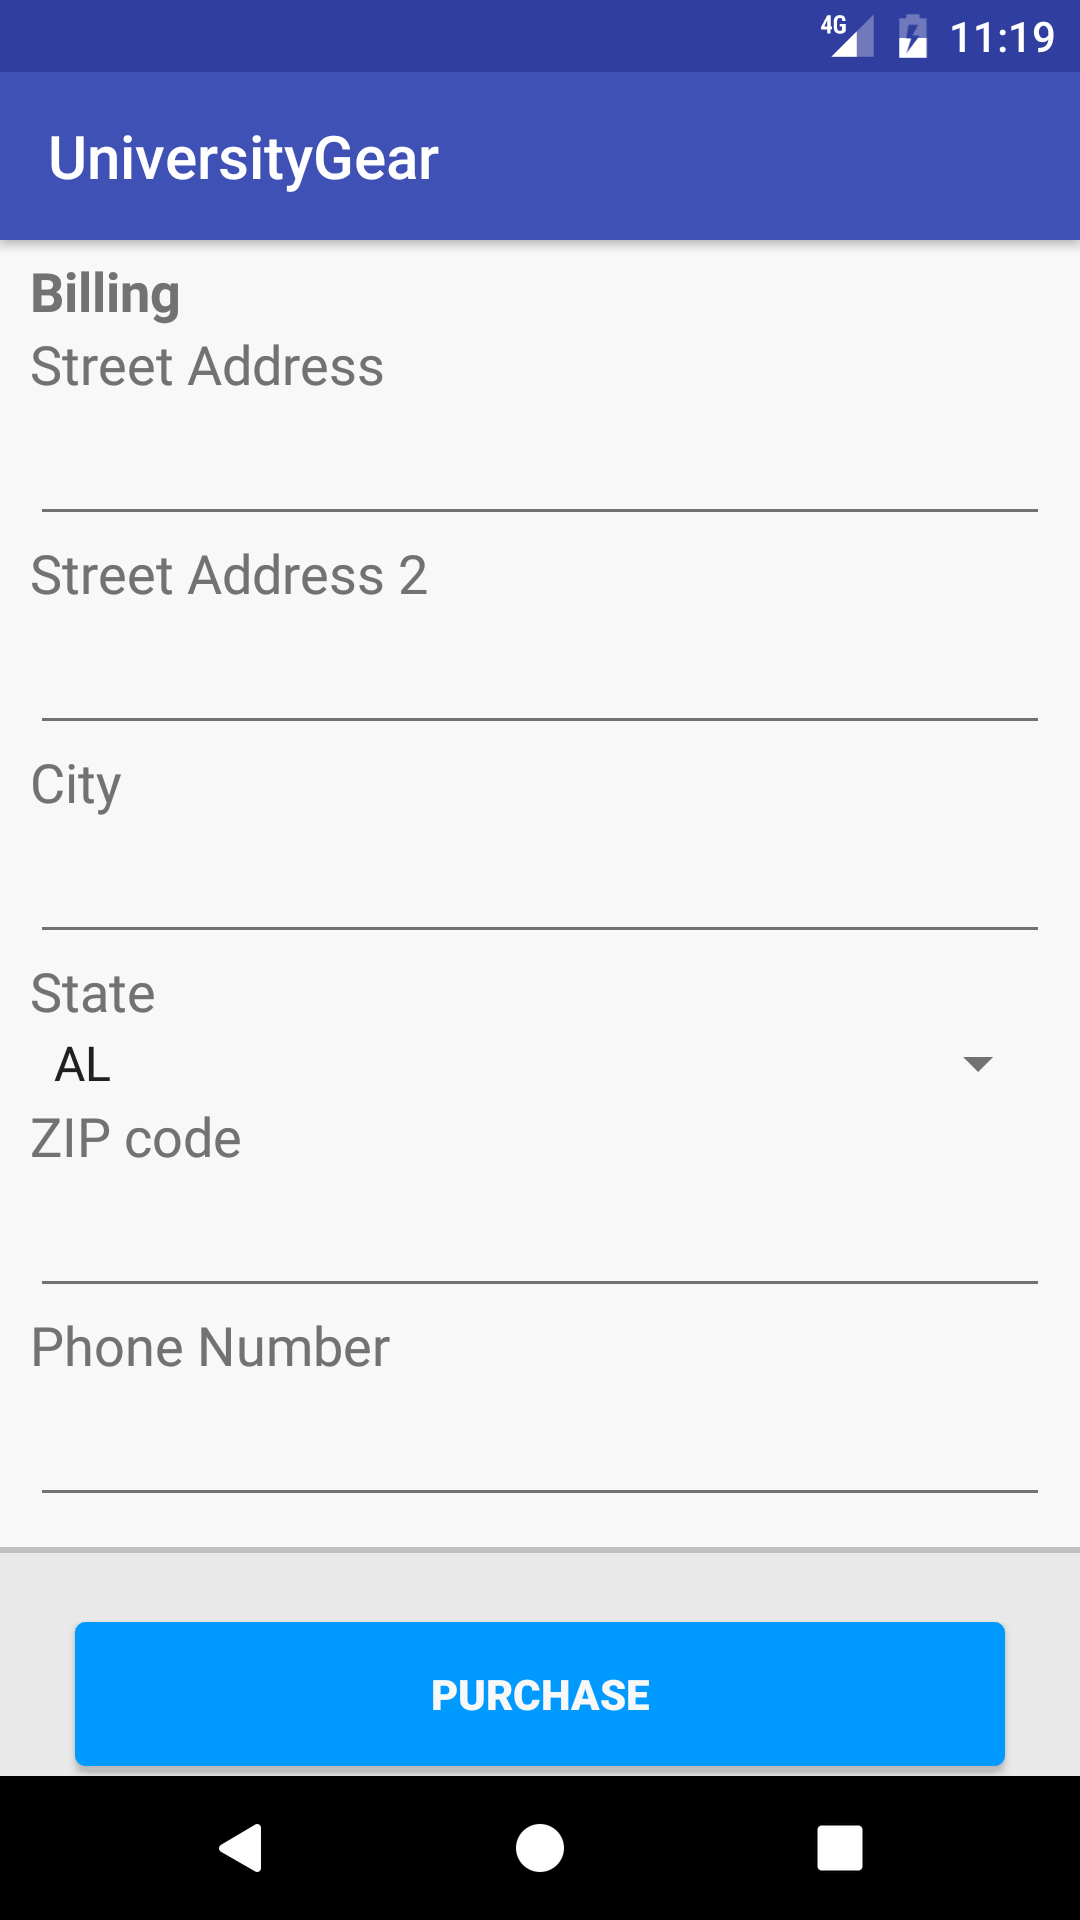
\includegraphics[scale=.2]{purchase}
\end{figure}
\FloatBarrier

\section{Retrospective}

\begin{table}[!ht]
\centering
\caption{Retrospectives}
\label{my-label}
\begin{tabularx}{\textwidth}{X|X|X}
\hline
\textbf{Positives} & \textbf{Deltas} & \textbf{Actions} \\ \hline
Completed the problem statement                  &  Didn't meet the criteria                &Rewrote the report to define the problem better                 \\ \hline
Met with the client in Portland                  &     Could meet with clients more frequently            & Arrange more meetings on-line                 \\ \hline
Completed the requirements document                  & Not quantifying goals, spelling errors, and missing an abstract                & Proofreading it more and asking for more clarifications prior to submitting it                 \\ \hline
Completed the technology review                 & Writing could be improved                & Go to the Writing Center in order to see missed mistakes                 \\ \hline
Completed the design document                  & Can start earlier                 &Talk more to TA and instructor on clarifying some matters                  \\ \hline
Complete the purchase class                       & Determine what causes the API error       & Use eBay's mentors as a better resource \\ \hline
Have group meetings more frequently        & Set strict meeting times                             & Hold members accountable for not meeting on time \\ \hline
\end{tabularx}
\end{table}

\FloatBarrier
\section{Conclusion}
So far, during the course of spring term, we have fully completed our application. 
The only things remaining are bug fixes. This means that so far, the team has completed
the requirements that were agreed upon in the fall. Some of the final bugs have also 
been found and have been fixed. 
 
\end{document}